% \documentclass[10pt,notes,mathserif]{beamer}
% \setbeameroption{show notes on second screen}
% \setbeamertemplate{note page}{\insertnote}

\documentclass[10pt,mathserif]{beamer}
\usepackage[utf8]{inputenc}

% Presentation specific stuff
\usetheme[progressbar=frametitle]{metropolis}
\usepackage[block=space,bibencoding=utf8,style=phys,maxbibnames=6,backend=biber]{biblatex}
\usepackage[font=footnotesize,labelformat=empty]{caption}
\usepackage{layouts}

% Math/physics notation stuff
\usepackage{amsmath}
\usepackage{amsfonts}
\usepackage{physics}
\usepackage{siunitx}
\usepackage{hyperref}
\usepackage{cleveref}
\usepackage{float}
\usepackage{stackengine}
\usepackage{calc}
\usepackage{xcolor}

% Misc
\usepackage[textsize=tiny,disable]{todonotes}
\usepackage{lipsum}

% Set up the biobliographies
\addbibresource{MPhys.bib}
\renewcommand*{\bibfont}{\tiny}
\setbeamerfont{bibliography item}{size=\tiny}
\setbeamerfont{bibliography entry author}{size=\tiny}
\setbeamerfont{bibliography entry title}{size=\tiny}
\setbeamerfont{bibliography entry location}{size=\tiny}
\setbeamerfont{bibliography entry note}{size=\tiny}

% Underlining, other notation and convenience commands
\stackMath
\newcommand{\suf}[2]{\stackunder[0.5pt]{\stackunder[1pt]{\ensuremath{#1}}{\rule{\widthof{\ensuremath{#2}}*\real{0.9}}{.1ex}}}{}}
\newcommand{\duf}[2]{\stackunder[0.5pt]{\stackunder[0.8pt]{\stackunder[1pt]{\ensuremath{#1}}{\rule{\widthof{\ensuremath{#2}}*\real{0.9}}{.1ex}}}{\rule{\widthof{\ensuremath{#2}}*\real{0.9}}{.1ex}}}{}}
\newcommand{\su}[1]{\suf{#1}{#1}}
\newcommand{\du}[1]{\duf{#1}{#1}}
\newcommand{\ssu}[1]{\scriptsize\su{#1}\normalsize}
\newcommand{\sdu}[1]{\scriptsize\du{#1}\normalsize}

\newcommand{\pp}{\ensuremath{\partial}}
\newcommand{\mgrad}{\ensuremath{\suf{\nabla}{K}\,}}
\newcommand{\QQ}{\ensuremath{\du{Q}}}
\newcommand{\nn}{\ensuremath{\su{n}}}
\newcommand{\NN}{\ensuremath{\su{N}}}
\newcommand{\MM}{\ensuremath{\su{M}}}
\newcommand{\EE}{\ensuremath{\du{E}}}
\newcommand{\PP}{\ensuremath{\du{\Pi}}}
\newcommand{\TT}{\ensuremath{\du{T}}}
\newcommand{\dudelta}{\ensuremath{\du{\delta}}}
\newcommand{\ddelta}[4]{\ensuremath{\delta_{#1#3}\delta_{#2#4} + \delta_{#1#4}\delta_{#2#3}}}
\newcommand{\PE}{\ensuremath{|\psi|_\text{eq}}}

\newcommand{\sL}{\ensuremath{\psi_\text{inplane}}}
\newcommand{\aL}{\ensuremath{\du{L}}}
\newcommand{\sP}{\ensuremath{\psi_\text{polar}}}
\newcommand{\aP}{\ensuremath{\du{P}}}

\newcommand{\FB}{\ensuremath{f_\text{bulk}}}
\newcommand{\FC}{\ensuremath{f_\text{comp}}}
\newcommand{\FU}{\ensuremath{f_\text{curv}}}

\newcommand{\onedot}{$\mathsurround0pt\ldotp$}
\newcommand{\cddot}{\mathbin{
    \vcenter{\baselineskip1ex \vspace{-0.1ex}\hbox{\onedot}\hbox{\onedot}}
}}

\newcommand{\extra}[1]{\color{gray} #1 \normalcolor}
\newcommand{\subheading}[1]{\large\textbf{#1}\normalsize}


\begin{document}

\setlength{\abovedisplayskip}{1em}
\setlength{\belowdisplayskip}{0ex}

% Motivation
\begin{frame}
    % \frametitle{E theory}
    \centering
    
\includegraphics[width=0.5\textwidth]{figures/PandA_black.pdf} \\
    \vspace{2em}
    \LARGE
    Complex Tensor Order Parameter for\linebreak Smectic Liquid Crystals \\
    \normalsize
    \vspace{0.5em}
    MPhys project 2023/24 \\

    \vspace{2em}

    \emph{Jan Kocka} \\
    \footnotesize supervised by \emph{Dr Tyler N Shendruk}

    \vspace{3em}

    \normalsize
    Main goals: adapt it for 3D \hspace{1ex}\&\hspace{1ex} new free energy form
\end{frame}

\begin{frame}[fragile]{Liquid crystals -- partial order in rod-like molecules}
    \newrefsection
    \begin{figure}
        \centering
        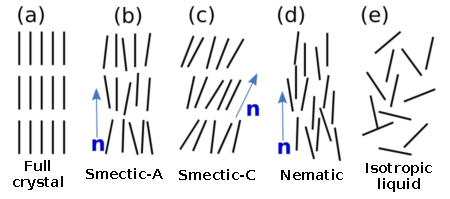
\includegraphics[width=0.9\textwidth]{figures/phases.pdf}
        \caption{
            Phases of a substance of rod-like molecules, in order of decreasing phase order\cite{pagetComplexTensorsSimple2023}.
        }
    \end{figure}
    \vspace{-1em}
    \bf
    Nematic $\sim$ alignment, broken rotational symmetry

    Smectic $\sim$ layering, broken translational symmetry in 1 direction
    \vfill
    \printbibliography[heading=none]
    \vspace{-\fill}
\end{frame}

\begin{frame}[fragile]{Liquid crystals -- why do we care?}
    \newrefsection
    \subheading{Physicists playground}
    \begin{itemize}
        \item Fascinating interplay of order and disorder
        \item Topological matter, various symmetries at play etc.
        \item Analogy between smectics and superconductivity\cite{degennesAnalogySuperconductorsSmectics1972}
    \end{itemize}
    \subheading{Real-world applications}
    \begin{itemize}
        \item Liquid crystal displays
        \item Organic electronics\cite{lagerwallNewEraLiquid2012}
        \item Biological and living matter\cite{lagerwallNewEraLiquid2012}
    \end{itemize}
    \vfill
    \printbibliography[heading=none]
    \vspace{-\fill}
\end{frame}

\begin{frame}[fragile]{Bacterial colonies have nematic and smectic order}
    \newrefsection
    \begin{figure}
        \centering
        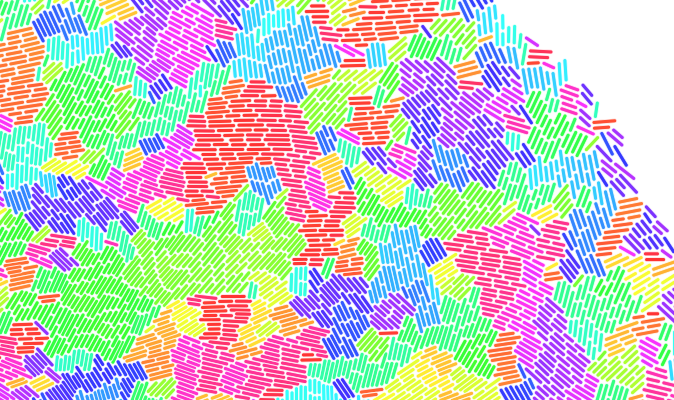
\includegraphics[width=\textwidth]{figures/bio_laila1.png}
        \caption{
            Example snapshot of a bacteria situation within the group.
            Colour shows the orientation of each bacterium.
            Domains of clear nematic and limited smectic order.
        }
    \end{figure}
    \vfill
    \printbibliography[heading=none]
    \vspace{-\fill}
\end{frame}

\begin{frame}[fragile]{Outline}
    \newrefsection
    \begin{itemize}
        \item Smectics as a density wave
        \item What \EE\ theory does better and how
        \item Constraints on \EE\ in 3D -- biaxiality
        \item Ginzburg-Landau dynamics
        \item New free energy
        \item Simulation results
    \end{itemize}
\end{frame}

\begin{frame}[fragile]{Layering is determined by three quantities}
    \newrefsection
    \begin{columns}
        \begin{column}{0.49\textwidth}
            \vspace{-\fill}
            \begin{center}
                \subheading{Smectic $\sim$ layered}
                \vspace{3em}

                \subheading{3 quantities \extra{(fields)}}
            \end{center}
            \begin{itemize}
                \item Degree of ordering
                \item Direction of layering % \extra{-- this has an additional symmetry}
                \item Spacing of layers
            \end{itemize}
        \end{column}
        \begin{column}{0.60\textwidth}
            \begin{figure}
                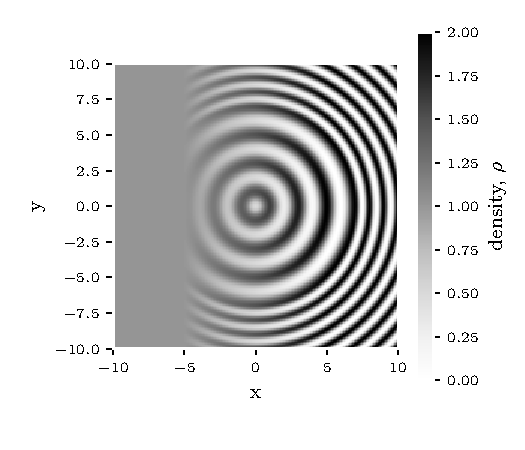
\includegraphics[width=\textwidth]{figures/layers_example.pdf}
                \caption{
                    Example of a layering structure
                }
            \end{figure}
        \end{column}
    \end{columns}
\end{frame}

\begin{frame}[fragile]{Layering as a density wave}
    \newrefsection
    \vspace{-1em}
    \begin{align*}
        \rho(\su{r}) &= \rho_0 + \rho_1\cos(\su{q_0}\cdot\su{r} + \phi) \\
        &= \rho_0 (1 + \Re(|\psi| e^{i(\ssu{q_0} \cdot \ssu{r} + \phi)})
    \end{align*}
    where
    \begin{itemize}
        \item $|\psi|$ is the wave amplitude -- degree of layering
        \item $\su{q_0}$ determines layering direction and spacing
        \begin{itemize}
            \item Layer normal direction $\NN=\frac{\ssu{q_0}}{q_0}$
            \item Layer spacing is $\frac{2\pi}{q_0}$
        \end{itemize}
        \item Here $\phi$ is an arbitrary phase
        % \item \textbf{Use complex order parameter $\psi = |\psi|e^{i\phi}$}
        \extra{\item $\rho_0$ is the average density and $\rho_1=\rho_0|\psi| \leq \rho_0$}
    \end{itemize}
\end{frame}

\begin{frame}[fragile]{Complex number order parameter $\psi(\su{r})$}
    \newrefsection
    \vspace{-\fill}
    \begin{align*}
        \rho(\su{r}) &= \rho_0 (1 + \Re(|\psi| e^{i(\ssu{q_0} \cdot \ssu{r} + \phi)}) \\
        &= \rho_0 (1 + \Re(\psi e^{i\ssu{q_0} \cdot \ssu{r}})
    \end{align*}
    \vspace{\fill}
    \begin{itemize}
        \item More interesting systems -- need to promote parameters to fields
        \item Promoting $|\psi|(\su{r})$ is simple
        \item $\phi(\su{r})$ also taken to be a field
        \item $\psi(\su{r}) = |\psi|(\su{r})e^{i\phi(\ssu{r})}$ is the de Gennes complex order parameter
    \end{itemize}
    \vspace{\fill}
    \printbibliography[heading=none]
    \vspace{-\fill}
\end{frame}

\begin{frame}[fragile]{Established approaches have problems}
    \newrefsection
    \vspace{-\fill}
    \begin{equation*}
        \rho(\su{r}) = \rho_0 (1 + \Re(\psi e^{i\ssu{q_0} \cdot \ssu{r}})
    \end{equation*}
    \vspace{\fill}

    \begin{columns}
        \begin{column}{0.49\textwidth}
            \subheadding{Two options, both limited}
            \begin{itemize}
                \item Fixed $\su{q_0}$, solve for $\psi(\su{r})$ -- near equilibrium systems only
                \item Remove $\su{q_0}$ -- does not capture the smectic $\NN\leftrightarrow-\NN$ symmetry\cite{pevnyiModelingSmecticLayers2014}
            \end{itemize}
        \end{column}
        \begin{column}{0.60\textwidth}
            \begin{figure}
                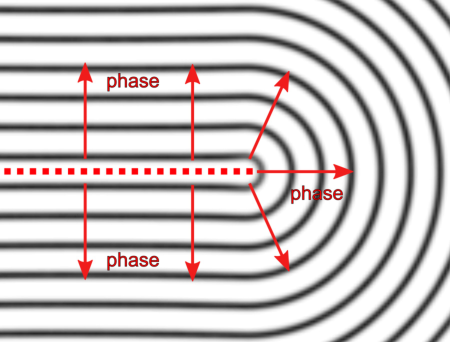
\includegraphics[width=0.8\textwidth]{figures/pevnyi.pdf}
                \caption{
                    Example density wave where the red arrows show directions of increasing $\phi$.
                    Black corresponds to layers of increased density.
                    Figure from \cite{pevnyiModelingSmecticLayers2014}.
                }
            \end{figure}
        \end{column}
    \end{columns}
    \vspace{\fill}
    \printbibliography[heading=none]
    \vspace{-\fill}
\end{frame}

% Intro to E
\begin{frame}[fragile]{E theory -- have varying \NN\ as well}
    \newrefsection
    Still use
    \begin{equation*}
        \rho(\su{r}) = \rho_0 (1 + \Re(\psi e^{i\ssu{q_0} \cdot \ssu{r}})
    \end{equation*}
    \vspace{-1.5em}
    \begin{itemize}
        \item Keep the $\psi(\su{r})$ field, and make $\NN(\su{r}) = \frac{\ssu{q_0}(\ssu{r})}{q_0}$ a field.
        \item Leave $\rho_0$, $q_0$ as microscopic constants
    \end{itemize}
    \vfill
    Package these as
    \begin{equation*}
        \du{E} = \psi(\su{N}\su{N} - \frac{\du{\delta}}{d})
    \end{equation*}
    \extra{where $d$ is the number of dimensions, 2 or 3}
\end{frame}

\begin{frame}[fragile]{E theory -- Mesoscopic theory respecting the layering symmetry}
    \newrefsection
    \vspace{-\fill}
    \begin{equation*}
        \du{E} = \psi(\su{N}\su{N} - \frac{\du{\delta}}{d})
    \end{equation*}
    \vfill

    \subheading{Benefits/motivation for \EE}
    \begin{itemize}
        \item Incorporates $\NN\leftrightarrow-\NN$ symmetry
        \item Captures all three quantities -- degree of order, layer direction and spacing through $|\psi|$, \NN\ and $\phi$
        \item Numerically convenient -- one object, it can numerically melt
        \extra{\item Mesoscopic theory -- does not directly resolve density}
    \end{itemize}
\end{frame}

\begin{frame}[fragile]{Treating \EE\ as our parameter requires constraints on it}
    \newrefsection
    \vspace{-\fill}
    \begin{equation*}
        \du{E} = \psi(\su{N}\su{N} - \frac{\du{\delta}}{d})
    \end{equation*}
    \vfill

    \begin{itemize}
        \item Treat \EE\ as general complex tensor
        \item Need to somehow enforce the form above
        % \item Real symmetric tensors adopt similar forms due to being diagonalizable
        \item Inspiration from real symmetric tensors leads us to diagonalization
        % \item Inspiration from $\du{Q}$ -- symmetric and traceless 
        % \begin{itemize}
        %     \item real so can be diagonalized
        % \end{itemize}
        \item Require $\du{E}$ be unitarily diagonalizable (\underline{normal}), \underline{symmetric} and \underline{traceless}
    \end{itemize}
\end{frame}

\begin{frame}[fragile]{Our constraints lead to biaxial \EE\ in 3D}
    \newrefsection
    Normality and tracelessness give \extra{in 3D}
    \begin{equation*}
        \du{E} = \du{U} \cdot \begin{pmatrix}
            \lambda_1 & 0 & 0 \\
            0 & \lambda_2 & 0 \\
            0 & 0 & \lambda_3 = - \lambda_1 - \lambda_2
        \end{pmatrix} \cdot \du{U}^\dagger
    \end{equation*}

    where the $\lambda_i$ are eigenvalues of \EE\ and $\du{U}$ a unitary matrix
\end{frame}

\begin{frame}[fragile]{Our constraints lead to biaxial \EE\ in 3D}
    \newrefsection
    Further using symmetry this fully implies
    \begin{equation*}
        \du{E} = \cdots = \psi_1(\su{N}}\su{N} - \frac{\du{\delta}}{3}) + \psi_2(\su{M}\su{M} - \frac{\du{\delta}}{3})
    \end{equation*}

    where
    \begin{align*}
        \psi_1 = \lambda_1 - \lambda_3 && \psi_2 = \lambda_2 - \lambda_3
    \end{align*}

    and \NN\ and \MM\ are real, mutually orthogonal unit eigenvectors of \EE\ associated to $\lambda_1$ and $\lambda_2$
\end{frame}

\begin{frame}[fragile]{Biaxial \EE\ could mean two density waves}
    \newrefsection
    \vspace{-\fill}
    \begin{equation*}
        \du{E} = \cdots = \psi_1(\su{N}}\su{N} - \frac{\du{\delta}}{3}) + \psi_2(\su{M}\su{M} - \frac{\du{\delta}}{3})
    \end{equation*}
    \vfill
    \begin{itemize}
        \item Symmetry, tracelessness, normality lead to biaxial \EE
        \item No simple way to force uniaxiality
        \item We interpret each term as a density wave
        \extra{\item This may allow \EE\ to model more ordered, columnar phases}
    \end{itemize}
\end{frame}

\begin{frame}[fragile]{Ginzburg-Landau theory -- dynamics by minimizing free energy}
    \newrefsection
    \begin{itemize}
        \item Dynamics using Ginzburg-Landau theory
        \item Need a free energy in terms of \EE
    \end{itemize}
    \begin{equation*}
        F = \int f(\du{E}, \mgrad\du{E}, \ldots) \dd{V}
    \end{equation*}
    \begin{itemize}
        \item $F$ must be real!
        \item Then evolve \EE\ to minimize $F$ using the functional derivative
    \end{itemize}
    \begin{equation*}
        \pdv{\du{E}}{t} = -\mu \fdv{F}{\EE^*}
    \end{equation*}
    \begin{itemize}
        \extra{\item Plus additional terms from Lagrange multipliers to enforce constraints}
    \end{itemize}
\end{frame}

% \begin{frame}[fragile]{The free energy}
%     \newrefsection
%     \begin{itemize}
%         \item $F$ must be real -- need to match $\du{E}$ and $\du{E}^*^$, simplest is
%     \end{itemize}
%     \begin{align*}
%         f_\text{bulk}(E_{ij}E_{ij}^* = \Tr(\du{E}\du{E}^*)) = A E_{ij}E_{ij}^* + \frac{C}{2} (E_{ij}E_{ij}^*)^2
%     \end{align*}
%     \begin{itemize}
%         \item \color{gray} In the uniaxial case $E_{ij}E_{ij}^* \propto |\psi|^2$, and $f_\text{bulk}$ corresponds to work of de Gennes \normalcolor
%     \end{itemize}
%     \begin{itemize}
%         \item Take the simplest gradients terms in one \EE
%     \end{itemize}
%     \begin{align*}
%         &|\su{\nabla}\du{E}|^2 = E_{ij,k}E_{ij,k}^* \\
%         &|\nabla^2\du{E}|^2 = E_{ij,kk}E_{ij,ll}^*
%     \end{align*}
% \end{frame}

\begin{frame}[fragile]{The one constant approximation free energy}
    \newrefsection
    \begin{align*}
        F &= \int f_\text{bulk} + f_\text{comp} + f_\text{curv} \dd{V} \\
        f_\text{bulk} &= A |\EE|^2 + \frac{C}{2} |\EE|^4 \\
        f_\text{comp} &= b_1 |\mgrad \EE|^2 \\
        f_\text{curv} &= b_2 |\nabla^2 \EE|^2
    \end{align*}
    \begin{itemize}
        \item \FB\ is the core free energy, determining the phase
        \item \FC\ corresponds to layer compression energy costs
        \item \FU\ corresponds to layer curvature/bending energy costs
        \extra{\item With $|?_{ij\ldots k}|^2=?_{ij\ldots k}?_{ij\ldots k}^*$ being the Frobenius norm}
    \end{itemize}
\end{frame}

\begin{frame}[fragile]{More complex $F$ using projection operators}
    \newrefsection
    \begin{itemize}
        \item Gradients in different directions have different energy costs
        \item For uniaxial \EE, special direction is $\su{N}$
        \item Projection operator $\du{\Pi}=\su{N}\su{N}$, rest is $\du{T} = \du{\delta} - \du{\Pi}$
        \extra{\item Consider $\su{\nabla} \rightarrow a \du{\Pi}\cdot\su{\nabla} + b \du{T}\cdot\su{\nabla}$ with $a, b$ being some constants}
    \end{itemize}

    \begin{align*}
        &f_\text{comp} \rightarrow b_1^\parallel \Pi_{kl} E_{ij,k}E_{ij,l}^* + b_1^\perp T_{kl} E_{ij,k}E_{ij,l}^* \\
        &f_\text{curv} \rightarrow b_2^\parallel \Pi_{kl}E_{ij,lk}\Pi_{mn}E_{ij,nm}^* + b_2^\perp T_{kl}E_{ij,lk}T_{mn}E_{ij,nm}^* \\
        &\phantom{f_\text{curv} \rightarrow}+ b_2^{\parallel\perp}(\Pi_{kl}E_{ij,lk}T_{mn}E_{ij,nm}^* + T_{kl}E_{ij,lk}\Pi_{mn}E_{ij,nm}^*)
    \end{align*}

    % \begin{equation*}
    %     \du{\Pi} =& \sqrt{\frac{d-1}{d \du{E} \cddot \du{E}}} \du{E} + \frac{\du{\delta}}{d} \\
    % \end{equation*}
\end{frame}

\begin{frame}[fragile]{The one constant approximation free energy}
    \newrefsection
    \begin{align*}
        F &= \int f_\text{bulk} + f_\text{comp} + f_\text{curv} \dd{V} \\
        f_\text{bulk} &= A |\EE|^2 + \frac{C}{2} |\EE|^4 \\
        f_\text{comp} &= b_1 |\mgrad \EE|^2 \\
        f_\text{curv} &= b_2 |\nabla^2 \EE|^2
    \end{align*}
    \begin{itemize}
        \item \FB\ is the core free energy, determining the phase
        \item \FC\ corresponds to layer compression energy costs
        \item \FU\ corresponds to layer curvature/bending energy costs
        \extra{\item With $|?_{ij\ldots k}|^2=?_{ij\ldots k}?_{ij\ldots k}^*$ being the Frobenius norm}
    \end{itemize}
\end{frame}

\begin{frame}[fragile]{Simple results -- \EE\ escapes into the third dimension}
    \newrefsection
    \begin{itemize}
        \item Fixed boundaries force \NN\ perpendicular to walls from sides
        \item Periodic boundaries in the third direction
        % \item I show a single slice
        \item Systems starts isotropic except a single streak
    \end{itemize}
\end{frame}

\begin{frame}[fragile]{Simple results -- \EE\ escapes into the third dimension}
    \newrefsection
    \begin{center}
        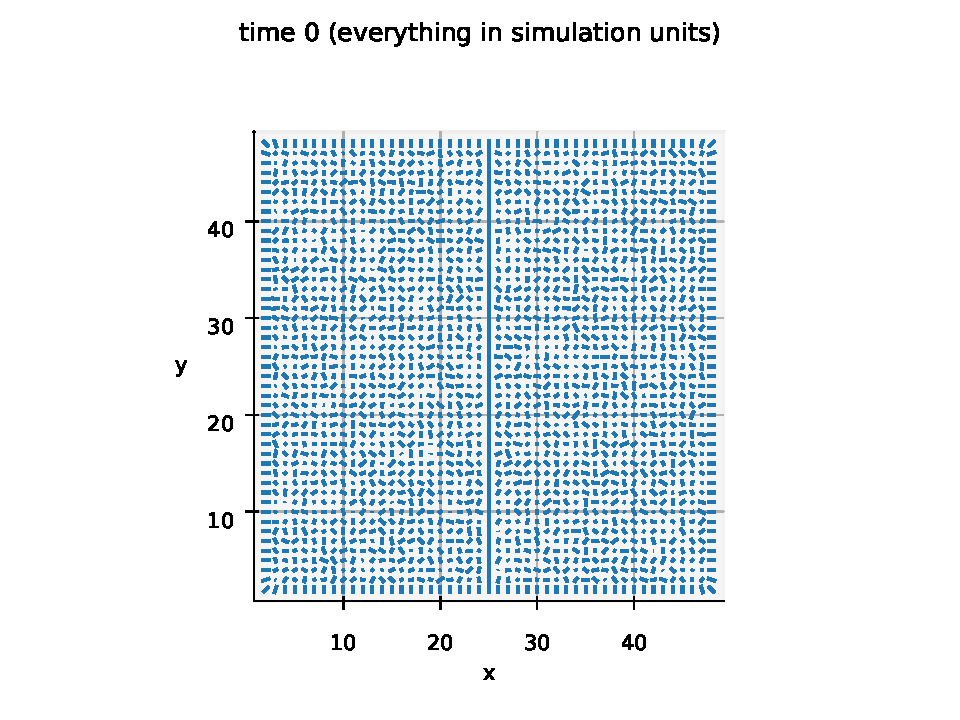
\includegraphics[width=\textwidth]{figures/prelim0.pdf}
    \end{center}
\end{frame}

\begin{frame}[fragile]{Simple results -- \EE\ escapes into the third dimension}
    \newrefsection
    \begin{center}
        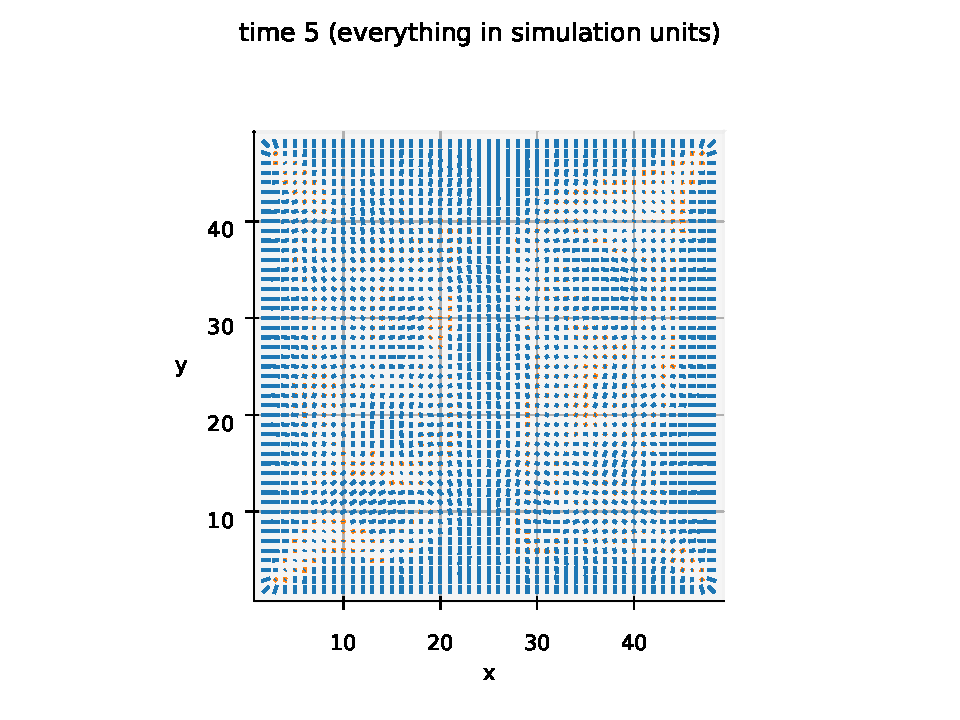
\includegraphics[width=\textwidth]{figures/prelim1.pdf}
    \end{center}
\end{frame}

\begin{frame}[fragile]{Simple results -- \EE\ escapes into the third dimension}
    \newrefsection
    \begin{center}
        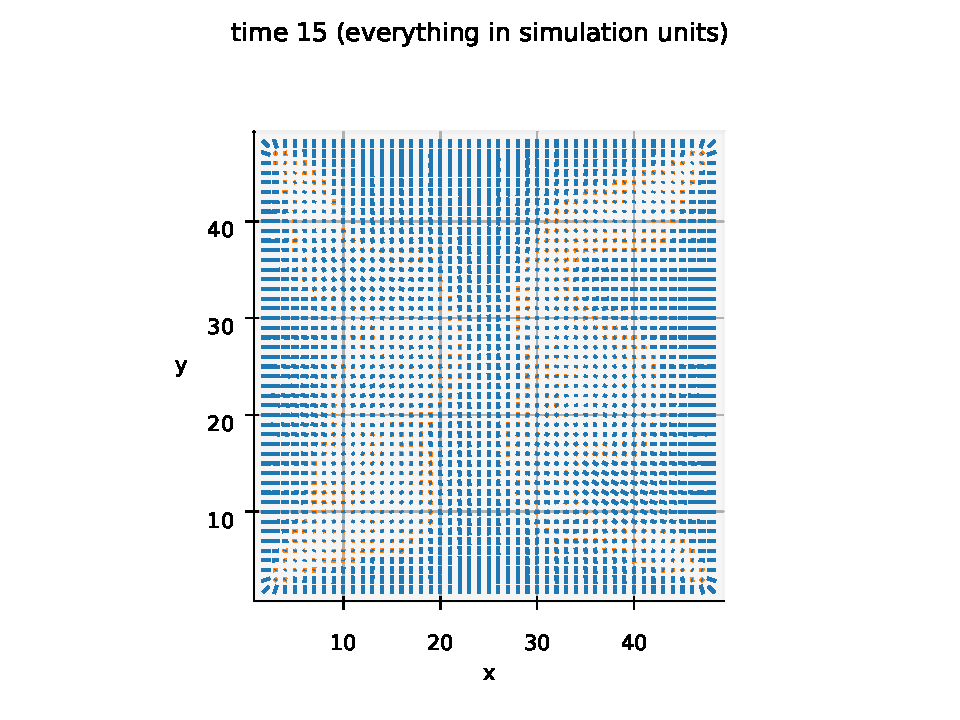
\includegraphics[width=\textwidth]{figures/prelim2.pdf}
    \end{center}
\end{frame}

\begin{frame}[fragile]{Simple results -- \EE\ escapes into the third dimension}
    \newrefsection
    \begin{center}
        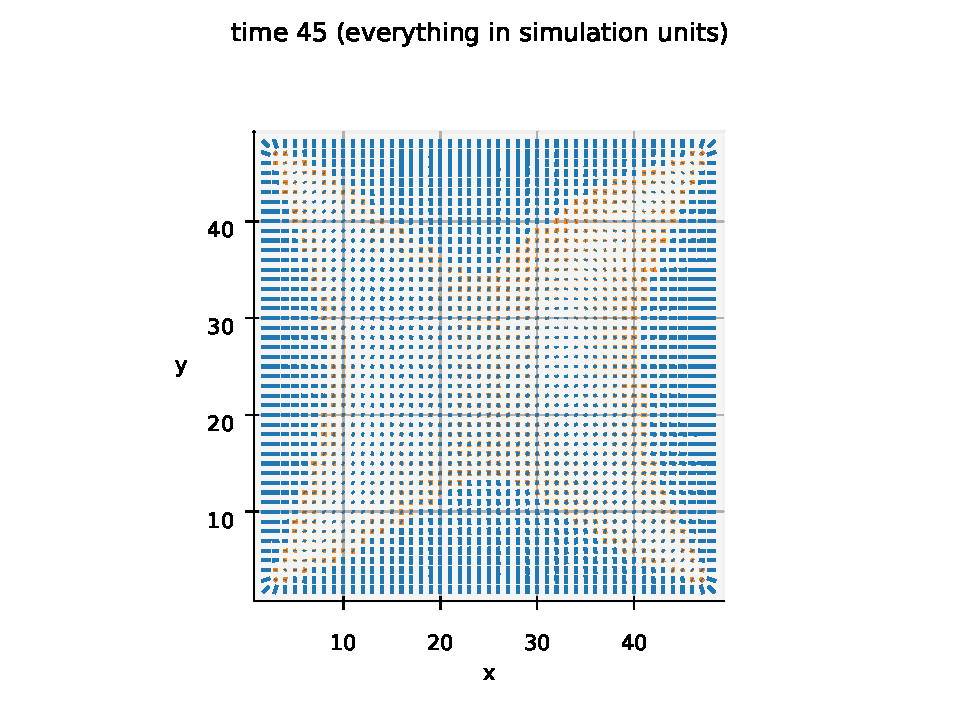
\includegraphics[width=\textwidth]{figures/prelim3.pdf}
    \end{center}
\end{frame}

\begin{frame}[fragile]{Simple results -- \EE\ escapes into the third dimension}
    \newrefsection
    \begin{center}
        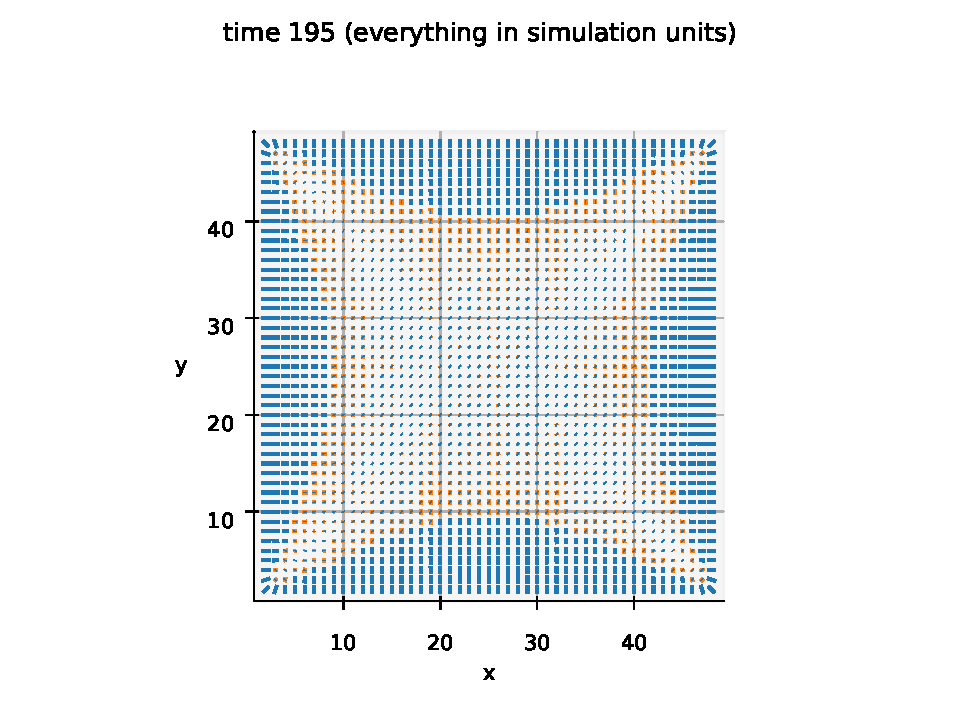
\includegraphics[width=\textwidth]{figures/prelim4.pdf}
    \end{center}
\end{frame}

\begin{frame}[fragile]
    \newrefsection
    \vspace{4em}
    \begin{center}
        \LARGE
        \textbf{Thank you for your attention}
    \end{center}
    \vspace{2em}
    \footnotesize
    \color{gray}
    \begin{align*}
        \fdv{F_\text{bulk}}{E_{ij}^*} =&\enspace \frac{1}{2}\qty(A + C E_{ab}E_{ab}^*)E_{ij} \\
        \fdv{F_\text{comp}}{E_{ij}^*} =&\enspace -(b_1^\parallel - b_1^\perp) (\Pi_{kl,l} E_{ij,k} + \Pi_{kl} E_{ij,kl}) - b_1^\perp E_{ij,kk} \\
        \fdv{F_\text{curv}}{E_{ij}^*} =&\enspace (b_2^\parallel + b_2^\perp - 2b_2^{\parallel\perp}) \Bigl( (\Pi_{kl}\Pi_{po,po} + 2\Pi_{kl,o}\Pi_{po,p} + \Pi_{kl,po}\Pi_{po})E_{ij,lk} \\
        &\phantom{\enspace (b_2^\parallel + b_2^\perp - 2b_2^{\parallel\perp}) \Bigl(}+ 2(\Pi_{kl,o}\Pi_{po} + \Pi_{kl}\Pi_{po,o})E_{ij,lkp} + \Pi_{kl}\Pi_{po}E_{ij,lkpo} \Bigr) \nonumber \\
        &+ (b_2^{\parallel\perp} - b_2^\perp)\Bigl( \Pi_{po,po}E_{ij,kk} + 2\Pi_{po,o}E_{ij,kkp} + \Pi_{po}E_{ij,kkpo} \nonumber \\ 
        &\phantom{\enspace+ (b_2^{\parallel\perp} - b_2^\perp)\Bigl(}+ \Pi_{kl,oo}E_{ij,lk} + 2\Pi_{kl,o}E_{ij,lko} + \Pi_{kl}E_{ij,lkoo} \Bigr) \nonumber \\ 
        &+ b_2^\perp E_{ij,kkoo} \nonumber
    \end{align*}
    \normalcolor\normalsize
\end{frame}

% Extras
\begin{frame}[fragile]{Liquid crystals -- partial order in rod-like molecules}
    \newrefsection
    \begin{figure}
        \centering
        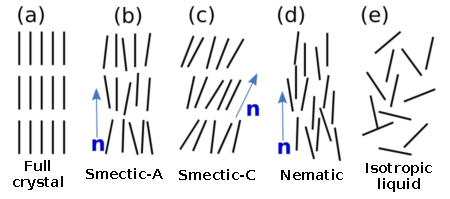
\includegraphics{figures/phases.pdf}
        \caption{
            Phases of a substance of rod-like molecules, in order of decreasing phase order\cite{pagetComplexTensorsSimple2023}.
        }
    \end{figure}
    \vspace{-0.5em}
    \normalsize\textbf{Different LC phases determined by their order/symmetries}\normalsize
    \vspace{-1.5em}
    \small
    \begin{table}
        \begin{tabular}{llll}
        Phase            & Order & Broken symmetry &  \\
        \hline
        Isotropic liquid & No order  & None &  \\
        Nematic          & Orientational & Rotational &  \\
        Smectic          & Positional & Translational in one direction & \\
        Full crystal     & Both & Rotational and translational in all directions &
        \end{tabular}
    \end{table}
    \vfill
    \printbibliography[heading=none]
    \vspace{-\fill}
    \note[itemize]{
        \item jaja
    }
\end{frame}

\begin{frame}[fragile]{$\psi(\su{r})$ alone does not respect smectic symmetry}
    \newrefsection
    \vspace{-\fill}
    \begin{equation*}
        \qq{here use} \rho(\su{r}) = \rho_0 (1 + \Re(|\psi| e^{i\phi})
    \end{equation*}
    \begin{figure}
        \centering
        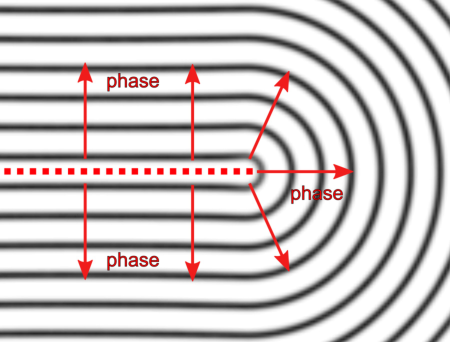
\includegraphics[width=0.6\textwidth]{figures/pevnyi.pdf}
        \caption{
            Example density wave where the red arrows show directions of increasing $\phi$.
            Black corresponds to layers of increased density.
            Figure from \cite{pevnyiModelingSmecticLayers2014}.
        }
    \end{figure}
    \printbibliography[heading=none]
    \vspace{-\fill}
\end{frame}

\begin{frame}[fragile]{Projection operators -- back to \EE}
    \newrefsection
    \begin{itemize}
        \item Need a form for \PP\ in terms of \EE
        \item Have 2 forms which work for uniaxial \EE
    \end{itemize}
    \begin{align*}
        \du{\Pi} =& \sqrt{\frac{d-1}{d \du{E} \cddot \du{E}}} \du{E} + \frac{\du{\delta}}{d} \\
        \du{\Pi} =& \frac{d-1}{d-2}\qty(\frac{\du{E} \cdot \du{E}^*}{\du{E} \cddot \du{E}^*} - \frac{\du{\delta}}{d(d-1)})
    \end{align*}
    \begin{itemize}
        \item First is significantly easier to work with -- currently used
        \color{gray}
        \item Lead to seemingly different functional derivatives -- why?
        \item First form only has $\du{E}$, how about $\du{E} \rightarrow \du{E}^*$?
        \item How well do they work for biaxial \EE?
        \normalcolor
    \end{itemize}
\end{frame}

\begin{frame}[fragile]{Dynamics of \EE}
    \newrefsection
    \begin{itemize}
        \item Want $\pdv{E_{ij}}{t} = -\mu\fdv{F}{E_{ij}^*}$ \color{gray} Model A like, \EE\ is not conserved \normalcolor
        \item But need constraints!
        \item Find extrema of $G$ instead
    \end{itemize}
    \begin{align*}
        G = \int f(\du{E}, \su{\nabla}\du{E}, \ldots) + \lambda_s g_s(\du{E}) + \lambda_t g_t(\du{E}) + \lambda_n g_n(\du{E}) \dd{V}
    \end{align*}
    \begin{itemize}
        \item Choose suitable $g$s and treat $\lambda$s as variables
    \end{itemize}
\end{frame}

\begin{frame}[fragile]{Lagrange multipliers}
    \newrefsection
    \begin{itemize}
        \item Choose real, non-negative $g_?(\du{E})$ that reflect the constraints:
    \end{itemize}
    \begin{align*}
        g_s &= |E_{ij} - E_{ji}|^2 \\
        g_t &= |E_{ii}|^2 \\
        g_n &= |[\du{E}, \du{E}^*]|^2 = |E_{ik}E_{kj}^* - E_{ik}^*E_{kj}|^2
    \end{align*}
    \begin{itemize}
        \item Two options for $\lambda$s -- soft constraints or approximate analytic form
        \item \color{gray} \EE\ is normal iff $[\du{E}, \du{E}^*] = 0$ \normalcolor
    \end{itemize}
\end{frame}

\begin{frame}[fragile]{Gradients of \PP}
    \newrefsection
    \begin{itemize}
        \item Results using the square root version of \PP
    \end{itemize}
    \scriptsize
    \begin{align*}
        \Pi_{kl} =&\enspace \frac{s E_{kl}}{\sqrt{E_{ab}E_{ab}}} + \frac{\delta_{kl}}{d} \\
        \Pi_{kl,m} =&\enspace \frac{s}{\sqrt{E_{ab}E_{ab}}} \qty(E_{kl,m} - \frac{E_{kl}E_{cd}E_{cd,m}}{E_{ab}E_{ab}}) \\
        \Pi_{kl,mn} =&\enspace \frac{s}{\sqrt{E_{ab}E_{ab}}} \Biggl(E_{kl,mn} \\ 
        &\phantom{\frac{s}{\sqrt{E_{ab}E_{ab}}} \Biggl(} -\frac{E_{kl,n}E_{cd}E_{cd,m} + E_{kl,m}E_{cd}E_{cd,n} + E_{kl}(E_{cd,n}E_{cd,m} + E_{cd}E_{cd,mn})}{E_{ab}E_{ab}} \\
        &\phantom{\frac{s}{\sqrt{E_{ab}E_{ab}}} \Biggl(} + 3\frac{E_{kl}E_{cd}E_{cd,m}E_{ef}E_{ef,n}}{(E_{ab}E_{ab})^2} \Biggr)
    \end{align*}
    \normalsize
\end{frame}

\begin{frame}[fragile]{Physical quantities}
    \newrefsection
    \begin{itemize}
        \item Taking $b_1$ to be the order of magnitude of $b_1^\parallel$ and $b_1^\perp$
        \item Similarly for $b_2$
    \end{itemize}
    \small
    \begin{align*}
        |\psi|_{eq} &= \sqrt{\frac{3}{2} * \frac{-A}{C}} \qq{The ideal smectic phase value, dimensionless}\\
        \varepsilon &= \sqrt{\frac{b_1}{|A|}} \qq{Lamellar in-plane coherence length, $L$} \\
        \lambda &= \sqrt{\frac{b_2}{b_1}} \qq{Penetration depth, $L$} \\
        \kappa &= \frac{\lambda}{\varepsilon} = \sqrt{\frac{b_2|A|}{b_1^2}} \qq{Ginzburg parameter, dimensionless}
    \end{align*}
\end{frame}

\end{document}
